\chapter{Raccolta dati ed analisi}
\vspace{0.5cm}
\label{cha:789}

Analizzando i diversi comportamenti della droplet nei vari esperimenti eseguiti e tenendo in considerazione che l'obiettivo di tale studio è quello di fare in modo che questa si muova velocemente e in maniera precisa lungo un percorso ipotizzato, si è cercata la combinazione ``migliore" dei parametri sperimentali che permettesse alla droplet di avvicinarsi il più possibile e nel minor tempo al punto in cui il sale è stato posto. Lo studio di questo movimento di chemiotassi, ci aiuterà a comprendere e a riprodurre le dinamiche di movimento delle cellule viventi.

\section{Esperimento con software}
L'esperimento precedentemente definito, viene ora eseguito per mezzo del programma sviluppato. Questo è stato creato utilizzando le API di EvoBot e sfruttando funzioni avanzate della libreria OpenCV.
Per portare a termine l'intero esperimento, l'operatore deve completare tre fasi: preparazione, raccolta dati, elaborazione dati. 

\subsection{Preparazione}
Per permettere al robot di accedere a liquidi e risorse esterne, bisogna posizionare sul piano degli esperimenti tutto ciò di cui potrebbe avere bisogno. Seguendo lo schema in figura, si posiziona (A) il decanolo, (B) il sale e (C) la Petri dish contenente uno strato di Decanoato.
\begin{figure}[h]
	  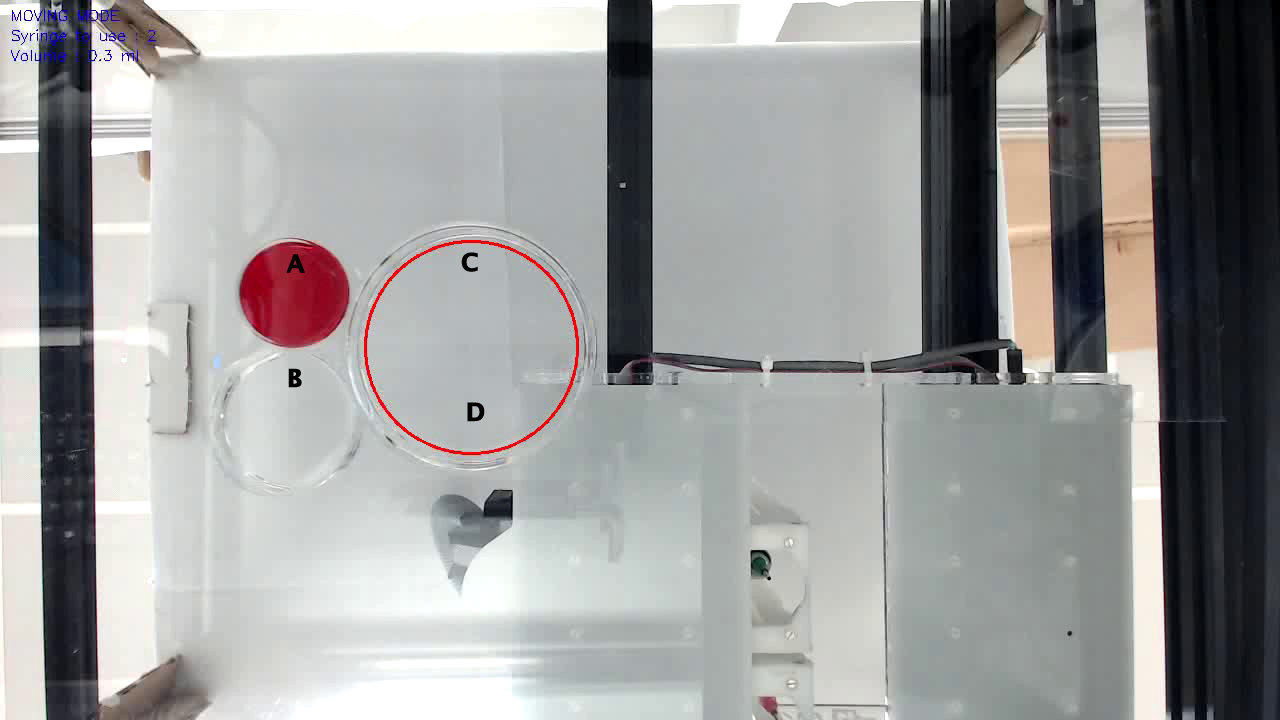
\includegraphics[scale=0.30]{immagini/exp1.jpg}
		\centering
	 \caption{experimental layout}
	\end{figure} 
\\Il protocollo seguito prevede cinque passaggi fondamentali: 
\begin{enumerate}

	\item Limitare l'area di interesse.\\
		La necessità di utilizzare Petri dish di diametri differenti e i problemi che possono essere causati da molteplici agenti esterni hanno suggerito che limitare la zona di interesse per ogni singolo esperimento potesse essere una soluzione: attraverso l'apposita interfaccia è possibile, quindi, disegnare un cerchio attorno alla Petri dish. Tutto ciò che si trova all'esterno di questo limite virtuale non verrà considerato dal programma.

	\item Prelevare $50\mu L$ di decanolo.\\
		Utilizzando una siringa delle due a disposizione, si raggiunge il pozzetto A, si fa scendere il corpo della stessa per prelevarne la quantità di decanolo richiesta. Bisogna tenere in considerazione che l'unità di volume che si può gestire è di $10\mu L$, grandezza nata dal compromesso tra avere un'interfaccia utilizzabile e una precisione accettabile. 

	\item Rilasciare $30\mu L$ di decanolo.\\
		 Posizionando la siringa precedentemente caricara sopra la Petri dish in poszione C, si rilascia il decanolo. 
La scelta di prelevare una quantità maggiore di quella richiesta ci assicura l'immissione nel sistema della corretta quantità in quanto può accadere che un volume non definito venga trattenuto nel corpo o nella punta della siringa.

	\item  Prelevare $500\mu L$ di NaCl. \\
		Utilizzando l'altra siringa, si raggiunge il pozzetto B e si eseguono le stesse azioni del punto 2, prelevando questa volta il sale. 
	
	\item Immettere $200\mu L$ di NaCl.\\
		Posizionando la siringa attualmente in uso sopra la Petri dish in posizione C, si rilascia il sale. 
\end{enumerate}



\subsection{Raccolta dati}
Fino ad ora l'utilizzo di EvoBot potrebbe risultare superfluo, è in questa fase che si può percepire il valore aggiunto che una macchina riesce ad apportare. Tramite l'utilizzo della webcam statica e la libreria di OpenCV, il programma permette di tracciare passo passo i movimenti della droplet, fino a 30 movimenti al secondo. Avere a disposizione i singoli punti dell'intero tracciato, permette di registrare qualsiasi particolare caratteristica che sarebbe sfuggita all'occhio umano. L'utilizzo che se ne può fare di questi punti è limitato dalla fantasia, si possono calcolare accelerazioni, \emph{pattern} oppure si possono comparare più percorsi dello stesso esperimento.
\\Nel nostro caso ci siamo limitati ad osservare se ci fosse un movimento della droplet verso il sale e si è cercato di capire in che ambiente questo risultasse più veloce e più preciso.
\\Per permettere alla webcam di riconoscere la droplet, questa è stata colorata di rosso grazie all'aggiunta del colorante Oil Red O alla soluzione di decanolo. Tuttavia, le droplet possono essere colorate non solo di rosso ma anche di altri colori, a seconda delle esigenze. Il programma mette a disposizione alcuni dei colori più utilizzati (come il rosso, il verde e il blu). 
\\ Per estrapolare informazioni dai dati raccolti durante l'esperimento, il programma si serve del salvataggio di questi su di un file \emph{.csv}.
Un esempio di questo file è disponibile nella tabella sottostante. 

\begin{center}
\begin{tabular}{lllllll}
X salt & Y salt & X droplet Start & Y droplet Start & X droplet End & Y droplet End & time(s) \\
\hline
405    & 418    & 378             & 300             & 425           & 434           & 88  
\end{tabular}
\end{center}


\subsection{Elaborazione dati}
I file prodotti durante la raccolta dati, vengono ora presi in carico da un altro programma che ha il compito di analizzare queste rilevazioni col fine di generare un unico file contenente dati e metadati dei singoli esperimenti.
\\La colonna più importante del file generato è quella che prende il nome di ``k". Questo coefficiente indica la precisione con cui la droplet si avvicina al sale ed è definita come:
\begin{equation} 	
	k := \frac { d(C,B) }{ d(A,C) }
\end{equation}
Dove A rappresenta il punto in cui la droplet viene trovata all'inizio del tracking , B quello in cui viene posizionato il sale, C dove la droplet si trova ad esperimento concluso, $d$ calcola la distanza euclidea tra i punti in questione. 
\\Possiamo assumere che più $d(C,B)$ tende a zero, più l'esperimento è preciso; da questo si evince che avere un $k$ tendente a zero è indice di successo.   
\begin{figure}[h]
	  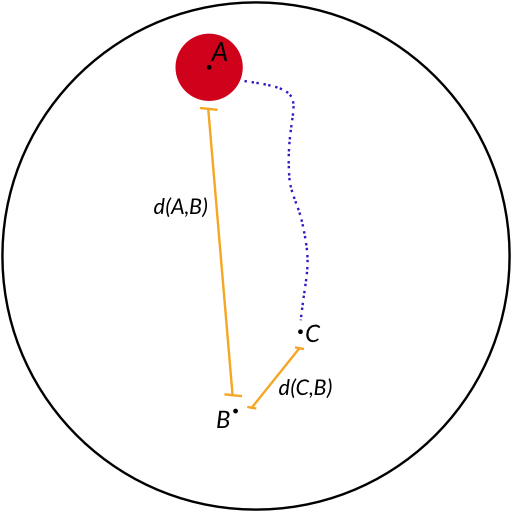
\includegraphics[scale=0.30]{immagini/schema.png}
		\centering
	 \caption{schema di un esperimento e degli elementi analizzati}
\end{figure} 
Una volta ottenuti tutti i $k$, mantenendo costante il $pH$ e le molarità, si vanno a calcolare tutti i $k$ medio per ogni singolo ambiente. L'ambiente rappresentato dal minor $k$ medio è quello che permette alla droplet di raggiungere il sale in maniera precisa e veloce. 
\\Durante la raccolta dati si è deciso di salvare anche il tempo impiegato dalla droplet nel movimento. Questo dato non viene utilizzato in questo studio ma potrà essere analizzato in studi futuri. 

\section{Risultati}
La soluzione di acido decanoico presente nella Petri prima dell'inizio dell'esperimento si presenta sottoforma di ione decanoato con carica negativa. Per disciogliere 20mM di acido decanoico in $1L$ di acqua abbiamo bisogno di aumentare il pH altrimenti l'acido resterebbe in forma solida. I risultati sono stati suddivisi per classi di molarità per rendere più semplice la lettura dei dati.

\subsection{20mM}
Nelle figure seguenti si osservano le droplet nelle tre condizioni differenti di pH. Nella soluzione di Decanoato con $pH11$ la droplet percorre un tratto più lungo e sono distinguibili il punto di inizio e il punto di fine. Per le altre due soluzioni non si può dire lo stesso, infatti i punti di inizio e fine del percorso risultano, se non coincidenti, molto vicini. 
\begin{figure}[h]
	\centering
   		{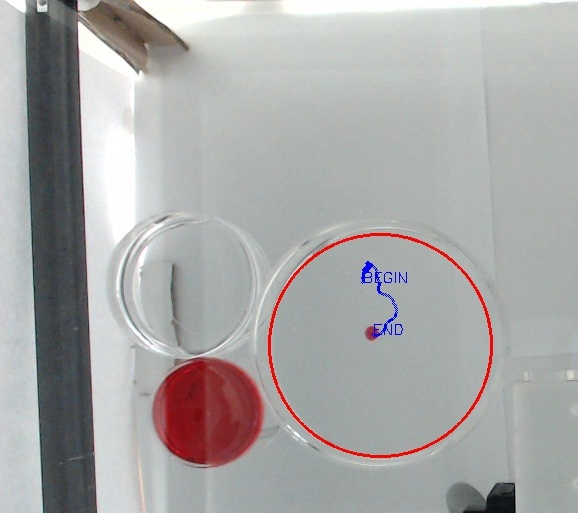
\includegraphics[width=5cm]{immagini/20mMpH11-2.jpg}} %ph11
 	\hspace{2mm}   	
		{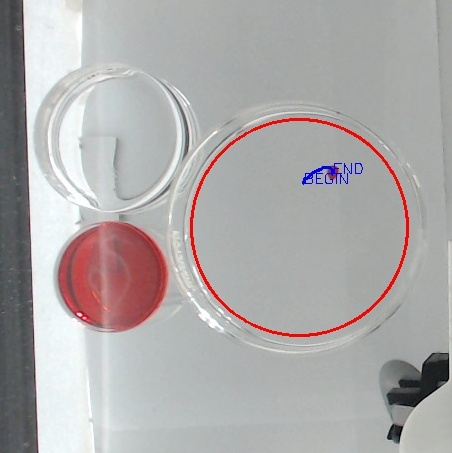
\includegraphics[width=5cm]{immagini/20mMpH12-2.jpg}}%ph12
	\hspace{2mm}   	
		{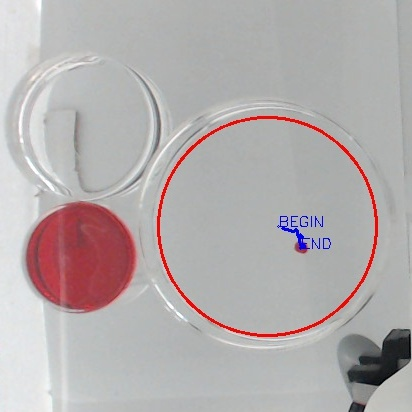
\includegraphics[width=5cm]{immagini/20mMpH13-2.jpg}}%ph13
	\caption{Acido decanoico 20mM a pH11, 12 e 13}
\end{figure}

Nella 




Nelle soluzioni con molarità $10mM$ e $5mM$ la droplet compie dei percorsi più lunghi, arrivando molto vicina al punto di inserimento del sale. Tutti i cammini mostrano una agitazione iniziale nel primo punto in cui la droplet viene riconosciuta. Questo movimento oscillatorio può essere dovuto alla prima interazione tra il sale ed le linee di confine della droplet.
Nelle figure 4.6 e 4.7 si possono osservare dei percorsi abbastanza analoghi tra loro, la droplet si avvicina in poco tempo in un punto prossimale al punto in cui il sale è stato inserito.
La tabella riportata di seguito mostra i risultati della funzione di \emph{fitness} per ognuno dei sei esperimenti. I valori  del coefficiente di precisione $k*$ sono stati trovati facendo al media dei risultati delle due ripetizioni. Si nota che il coefficiente migliore è quello della soluzione con molarità $5mM$, con un valore di 11,413.


\subsection{10mM}
\begin{figure}[h]
	\centering
   		{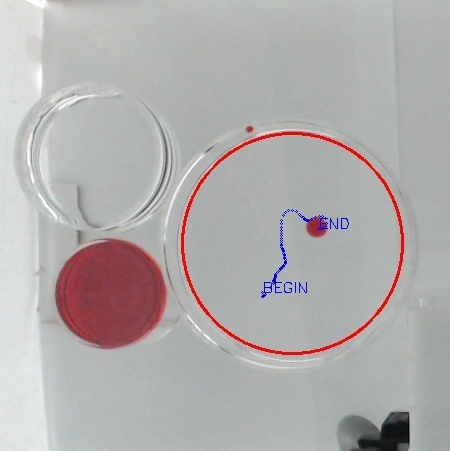
\includegraphics[width=5cm]{immagini/10mMph11-2.jpg}} %ph11
 	\hspace{2mm}   	
		{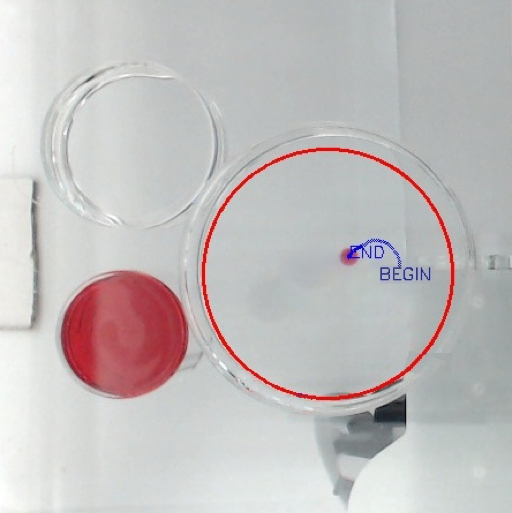
\includegraphics[width=5cm]{immagini/10mMpH12-1.png}} %PH 12
	\hspace{2mm}   	
		{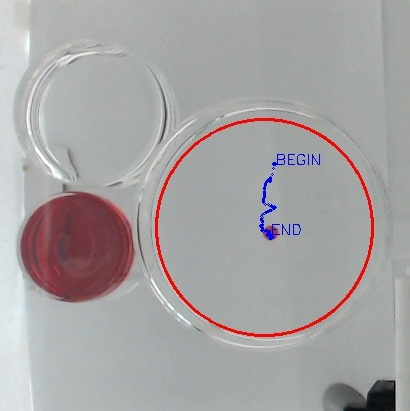
\includegraphics[width=5cm]{immagini/10mMpH13-2.jpg}}  %PH 13
	\caption{Acido decanoico 10mM a pH11, 12, 13}
\end{figure}

\begin{center}
\begin{tabular}{lll}
pH & k     & tempo (s) \\
11 & 0,671 & 135       \\
11 & 0,074 & 41        \\
11 & 0,538 & 116       \\
11 & 0,209 & 52        \\
12 & 0,566 & 85        \\
12 & 0,241 & 46        \\
12 & 0,763 & 96        \\
12 & 0,447 & 62        \\
13 & 0,876 & 79        \\
13 & 0,338 & 40        \\
13 & 0,732 & 61        \\
13 & 0,424 & 49       
\end{tabular}
\end{center}


\begin{center}
\begin{tabular}{llll}
pH	& k medio	& tempo (s)	& ks medio\\
11	& 0,373	& 86	& 32,078\\
12	& 0,50425	& 72,25	& 36,4320625\\
13	& 0,5925	& 57,25	& 33,920625
\end{tabular}
\end{center}


gfcdxhshdrjftkgjhkl.
Tutte le soluzioni con $pH12$ portano a risultati simili. Si osserva che la droplet non compie uno spostamento lineare determinante.
La tabella riportata di seguito mostra i risultati della funzione di \emph{fitness} per ognuno dei sei esperimenti. I valori del coefficiente di precisione $k*$ sono stati trovati facendo al media dei risultati delle due ripetizioni.


La condizione di stabilità della droplet può essere dovuta a due fattori estranei al sistema. Infatti la droplet può essere stata influenzata dai moti convettivi creati dall'inserimento della punta della siringa all'interno della superficie dell'acido decanoico nella Petri o dagli spostamenti di aria attorno al robot. Tuttavia, queste ipotesi non possono essere confermate a causa del basso numero di ripetizioni dell'esperimento. 






\subsection{5mM}

\begin{figure}[h]
	\centering
   		{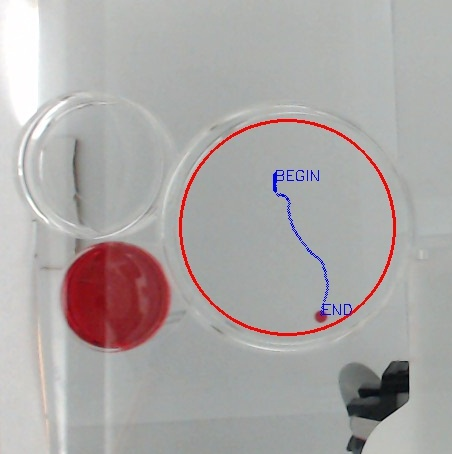
\includegraphics[width=5cm]{immagini/5mMpH11-1.jpg}} %ph11
 	\hspace{2mm}   	
		{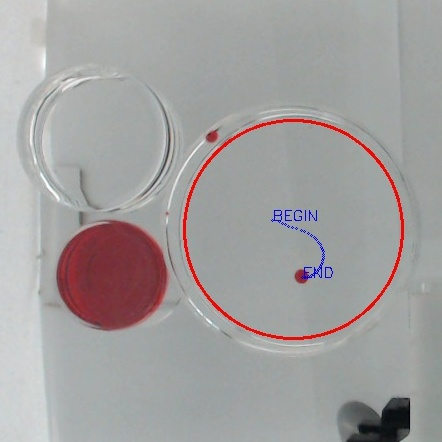
\includegraphics[width=5cm]{immagini/5mMpH11-2.jpg}}%ph12
	\hspace{2mm}   	
		{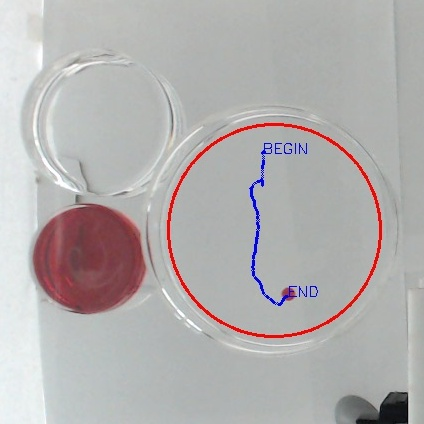
\includegraphics[width=5cm]{immagini/5mMpH13-2.jpg}}%ph13
	\caption{Acido decanoico 5mM a pH11, 12 e 13}
\end{figure}




\\Gli esperimenti a $pH$ maggiore hanno dimostrato che la droplet si muove con più facilità e percorrendo un percorso più lineare a molarità minori. 
La tabella riportata di seguito mostra i risultati della funzione di \emph{fitness} per ognuno dei sei esperimenti. I valori del coefficiente di precisione $k*$ sono stati trovati facendo al media dei risultati delle due ripetizioni. 


\subsection{Considerazioni generali}
In tutti i casi analizzati si è osservato, una volta che la droplet si avvicina al punto in cui è stato inserito il sale, che questa compie un movimento locale casuale ed oscillatorio.
Inoltre è stato notato che la droplet non risponde con un movimento chemiotattico immediatamente dopo l'aggiunta del sale. Probabilmente questo periodo di latenza 


\begin{center}
\begin{tabular}{lllllllll}
pH & mol (mM) & \# esp & k           & k medio     & tempo (s) & tempo medio (s) & k* ∀ molarità & k* ∀ pH     \\
11 & 5            & 1              & 0,180 & 0,215 & 87        & 53              & 11,413   &             \\
11 & 5             & 2              & 0,250 &             & 19        &                 &               &             \\
11 & 10            & 1              & 0,530 & 0,302 & 135       & 88              & 26,612   & 11,413 \\
11 & 10            & 2              & 0,074 &             & 41        &                 &               &             \\
11 & 20            & 1              & 0,453 & 1,991 & 205       & 166,5           & 331,594   &             \\
11 & 20            & 2              & 3,529 &             & 128       &                 &               &            
\end{tabular}
%\caption{Tabella risultati delle soluzioni a pH11}
\end{center}

\begin{center}
\begin{tabular}{lllllllll}
pH & mol (mM) & \# esp & k      & k medio & tempo (s) & tempo medio (s) & k* ∀ molarità & k* ∀ pH \\
13 & 5        & 1      & 0,175  & 0,325   & 63        & 59              & 19,182        &         \\
13 & 5        & 2      & 0,474  &         & 55        &                 &               &         \\
13 & 10       & 1      & 0,876  & 0,607   & 61        & 82              & 49,820        & 19,182  \\
13 & 10       & 2      & 0,338  &         & 103       &                 &               &         \\
13 & 20       & 1      & 31,231 & 16,351  & 70        & 74              & 1210,032      &         \\
13 & 20       & 2      & 1,472  &         & 78        &                 &               &     
\end{tabular}
\end{center}


\begin{center}
\begin{tabular}{lllllllll}
pH & mol (mM) & \# esp & k           & k medio     & tempo (s) & tempo medio (s) & k* ∀ molarità & k* ∀ pH     \\
12 & 5             & 1              & 1,837 & 1,170 & 214       & 143,5           & 168,026    \\
12 & 5             & 2              & 0,504 &             & 73        &                 &               &             \\
12 & 10            & 1              & 0,566 & 0,403 & 85        & 65,5            & 26,443   & 26,443 \\
12 & 10            & 2              & 0,241 &             & 46        &                 &               &             \\
12 & 20            & 1              & 4,075 & 3,407 & 77        & 84,5            & 287,957   &             \\
12 & 20            & 2              & 2,740 &             & 92        &                 &               &            
\end{tabular}
\end{center}
















